\documentclass{beamer} \usepackage{amsmath,amsthm}
\usepackage{graphicx,microtype,parskip}
\usepackage{caption,subcaption,multirow}
\usepackage{attrib}

\frenchspacing

\usetheme{default}
\usecolortheme{whale}

\setbeamertemplate{navigation symbols}{}

\setbeamercolor{title}{fg=blue,bg=white}

\setbeamercolor{block title}{fg=white,bg=gray}
\setbeamercolor{block body}{fg=black,bg=lightgray}

\setbeamercolor{block title alerted}{fg=white,bg=darkgray}
\setbeamercolor{block body alerted}{fg=black,bg=lightgray}

\AtBeginSection[]
{
  \begin{frame}
    \tableofcontents[currentsection]
  \end{frame}
}


\title{Evolutionary paleoecology and\\ the biology of extinction}
\author{Peter D Smits}
\institute{Committee on Evolutionary Biology, University of Chicago}

\begin{document}

\begin{frame}
  \maketitle
\end{frame}

\begin{frame}
  \tableofcontents
\end{frame}


\section{Introduction and theory}

\begin{frame}
  \frametitle{Framework}

  \begin{alertblock}{Questions}
    \begin{itemize}
      \item Why do certain taxa go extinct while others do not?
      \item How is emergence ``formed?'' When should it be invoked?
      \item Is extinction risk taxon--age independent?
      \item When should we expect global, regional, or local processes to dominate?
    \end{itemize}
  \end{alertblock}
  
\end{frame}

\begin{frame}
  \frametitle{Evolutionary paleoecology}
  \begin{quotation}
    \dots the consequences of distinct ecological factors on differential rate dynamics, particularly rates of faunal turnover and diversification.

    \tiny{\attrib{Kitchell 1985 \textit{Paleobiology}}}
  \end{quotation}

  \vspace{1.3cm}

  \begin{center}
    environmental interactions \(\rightarrow\) macroevolution
  \end{center}
\end{frame}

\begin{frame}
  \frametitle{Emergent properties}

  \begin{center}
    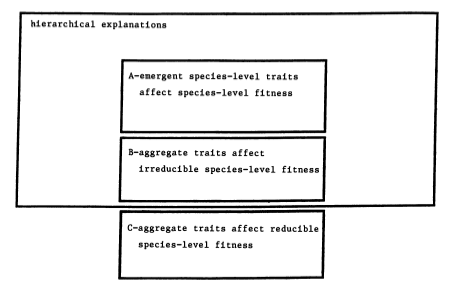
\includegraphics[height=0.4\textheight, width=\textwidth, keepaspectratio=true]{figure/grantham}

    \tiny{\attrib{Grantham 1995 \textit{Ann. Rev. Ecol. Syst.}}}
  \end{center}

  \begin{block}{Species level}
    Trait that cannot be reduced to organismal level
    
    Product of one or more traits/factors
  \end{block}

\end{frame}

\begin{frame}
  \frametitle{Range size}
  
  \begin{center}
    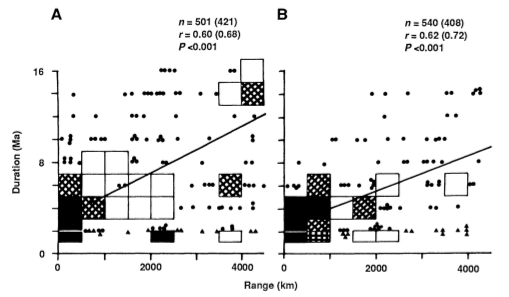
\includegraphics[height = 0.8\textheight, width = \textwidth, keepaspectratio = true]{figure/range}

    \tiny{\attrib{Jablonski 1987 \textit{Science}}}
  \end{center}
\end{frame}

\begin{frame}
  \frametitle{Probability of survival}

  \begin{columns}
    \begin{column}{0.5\textwidth} 
      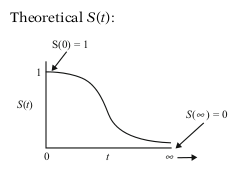
\includegraphics[height = 0.4\textheight, width = \textwidth, keepaspectratio = true]{figure/ideal}

      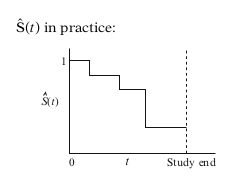
\includegraphics[height = 0.4\textheight, width = \textwidth, keepaspectratio = true]{figure/prac}

      \tiny{\attrib{Kleinbaum and Klein 2012}}
    \end{column}
    \begin{column}{0.5\textwidth}
      \begin{block}{Survival function}
        \[
          S(t) = P(T > t)
        \]

        \begin{itemize}
          \item \(T\): survival time (\(\geq 0\))
          \item \(t\): specified time 
        \end{itemize}
      \end{block}
    \end{column}
  \end{columns}
\end{frame}

\begin{frame}
  \frametitle{Instantaneous potential of failure (extinction)}

  \begin{block}{Hazard function \(\equiv\) conditional failure rate}
    \[
      h(t) = \lim_{\Delta t \to 0} \frac{P(t \leq T < t + \Delta t | T \geq t)}{\Delta t}
    \]
  \end{block}

  \begin{center}
    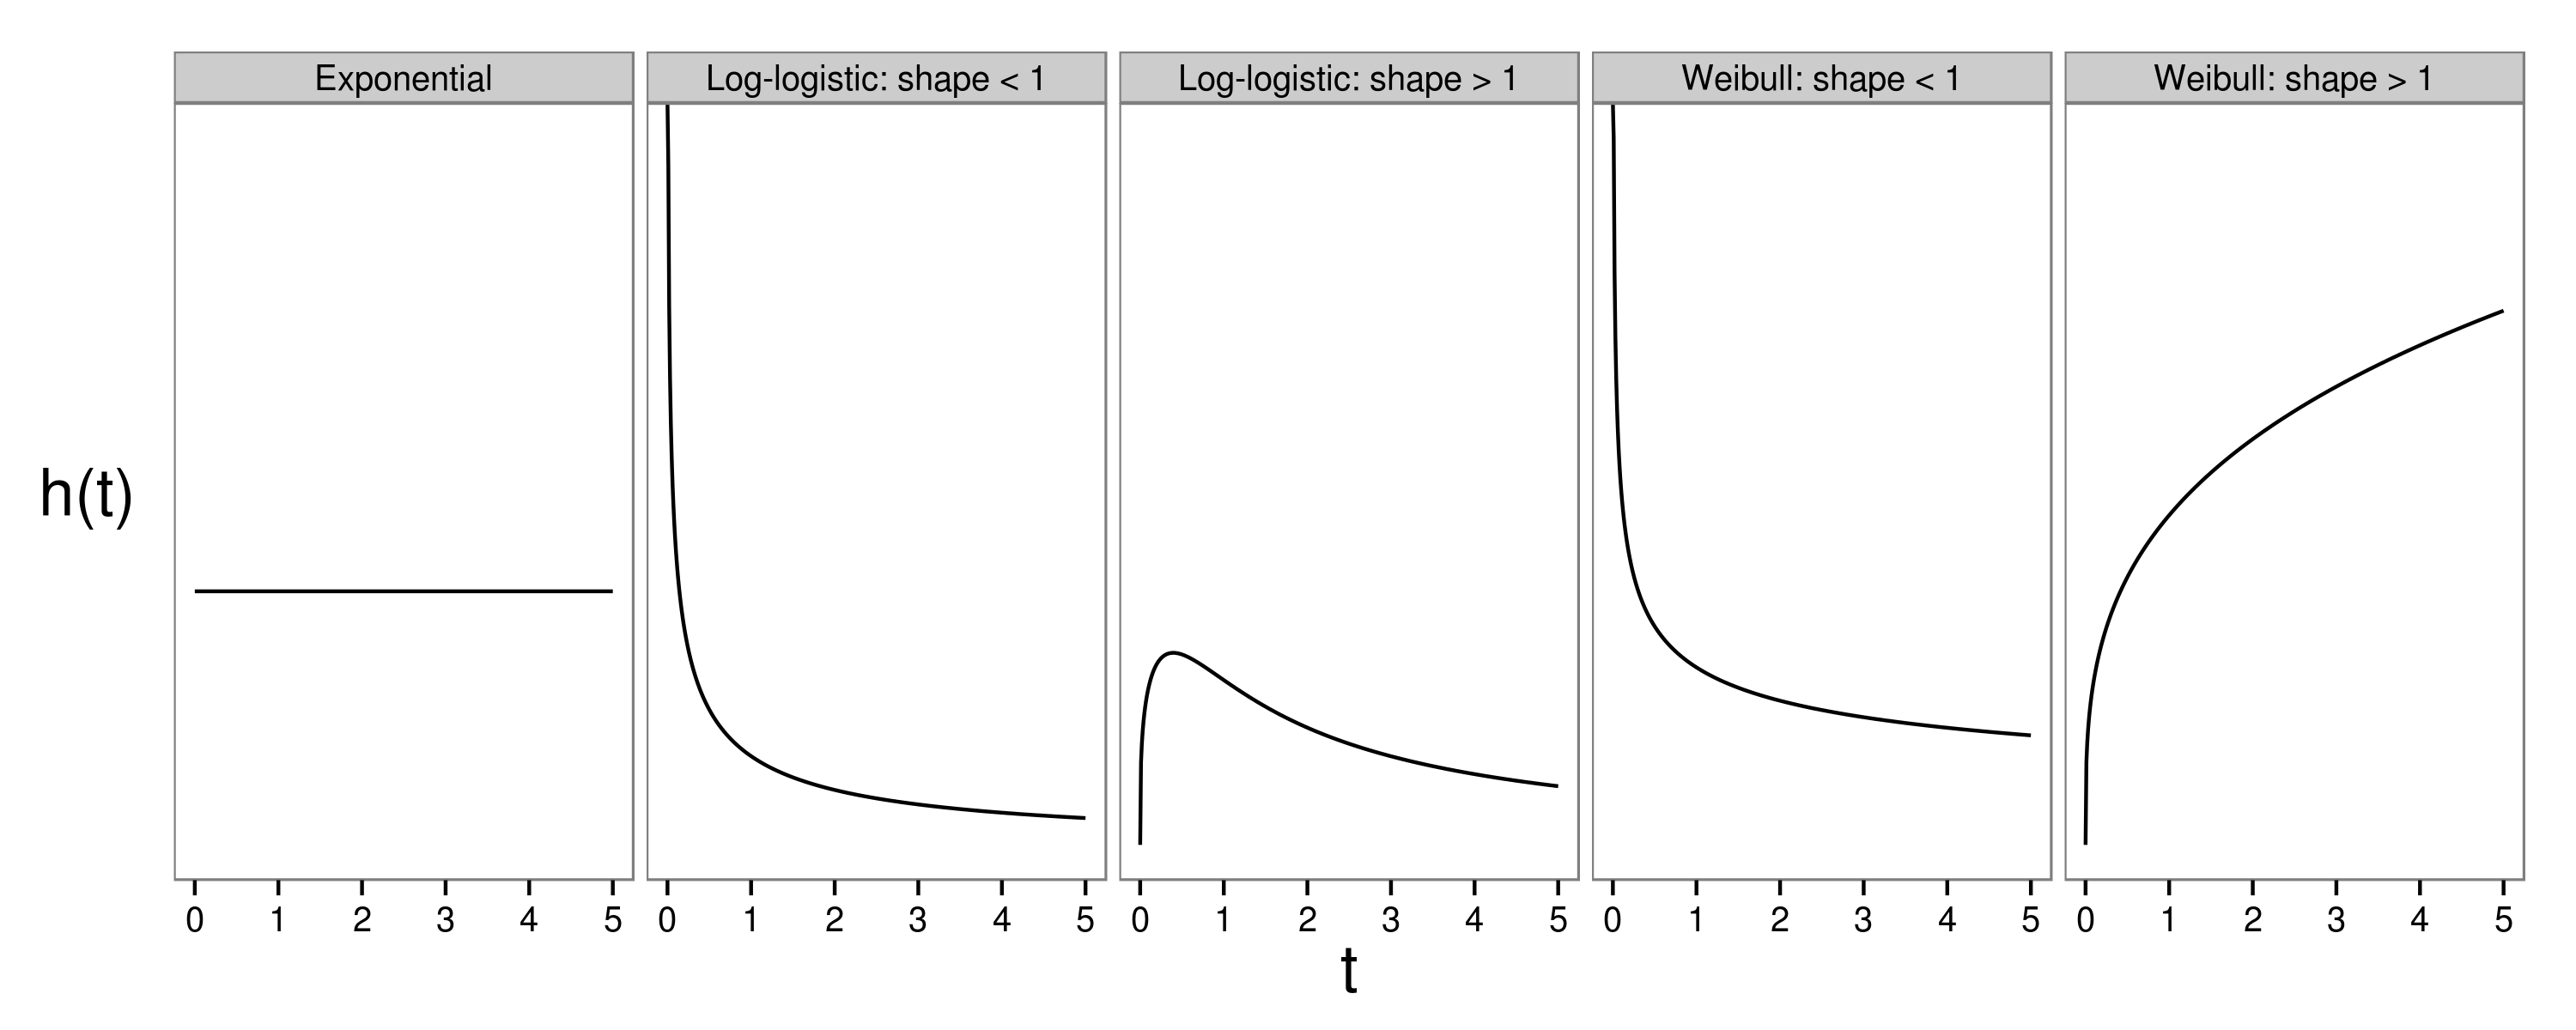
\includegraphics[height = 0.5\textheight, width = \textwidth, keepaspectratio = true]{figure/hazard}
  \end{center}
\end{frame}

\begin{frame}
  \frametitle{Van Valen's observation of survival}

  \begin{center}
    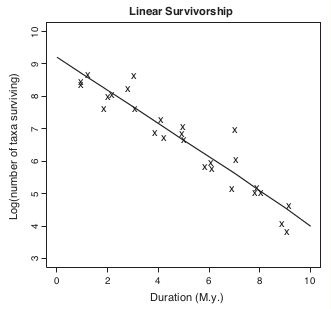
\includegraphics[height = 0.7\textheight, keepaspectratio = true]{figure/liow}

    \tiny{\attrib{Liow et al. 2011 \textit{TREE}}}
  \end{center}
\end{frame}

\begin{frame}
  \frametitle{Law of Constant Extinction}

  \begin{alertblock}{Definition}
      Extinction risk in a given adaptive zone is taxon--age independent.

      \tiny{\attrib{Van Valen 1973 \textit{Evol. Theory}}}
  \end{alertblock}

  \begin{center}
    translation: hazard is constant with respect to time \\(\alert{exponential survival})
  \end{center}

  \[
    h(t) = \lambda \iff S(t) = \exp^{-\lambda t}
  \]

\end{frame}

\begin{frame}
  \frametitle{Brachiopods and mammals: a comparison}

  \begin{columns}
    \begin{column}{0.5\textwidth}
      \begin{block}{brachiopods}
        \begin{itemize}
          \item marine
          \item sessile
          \item Permian (\(\sim 47\) My)
          \item Australasia
          \item global warming
        \end{itemize}
        % tattoo
      \end{block}
    \end{column}
    \begin{column}{0.5\textwidth}
      \begin{block}{mammals}
        \begin{itemize}
          \item terrestrial
          \item motile
          \item Cenozoic (\(\sim 65\) My)
          \item North America, Europe, South America
          \item global cooling
        \end{itemize}
        % annyong
      \end{block}
    \end{column}
  \end{columns}
\end{frame}

\begin{frame}
  \frametitle{Series of related questions}

  \begin{itemize}
    \item generic level survival in brachiopods %and mammals
      \begin{itemize}
        \item ecological traits re. environmental pref. (emergence)
        \item survival distribution
      \end{itemize}
    \item specific level survival in mammals
      \begin{itemize}
        \item ecological traits re. range size (emergence)
        \item generic versus specific survival
        \item anagenesis/species:genus simulation
        \item survival distribution
      \end{itemize}
    \item community connectedness in mammals
      \begin{itemize}
        \item global versus regional versus local scale processes
        \item ecological traits (trophic/locomotion)
      \end{itemize}
  \end{itemize}
\end{frame}


\section{Brachiopods, environmental preference, and extinction}

\begin{frame}
  \frametitle{Traits relating to environment and range size}

  \begin{itemize}
    \item substrate affinity
      \begin{itemize}
        \item physical, chemical
        \item availability
      \end{itemize}
    \item habitat preference
      \begin{itemize}
        \item energetics
        \item availability
      \end{itemize}
    \item affixing strategy
      \begin{itemize}
        \item energetics
        \item optimality
      \end{itemize}
  \end{itemize}
\end{frame}

\begin{frame}
  \frametitle{Substrate affinity}

  \begin{columns}
    \begin{column}{0.5\textwidth}
      \begin{center}
        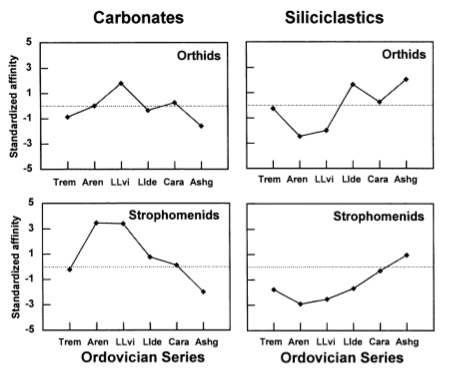
\includegraphics[height = 0.4\textheight, keepaspectratio = true]{figure/miller}
          
        \tiny{\attrib{Miller and Connoly 2001 \textit{Paleobio.}}}

        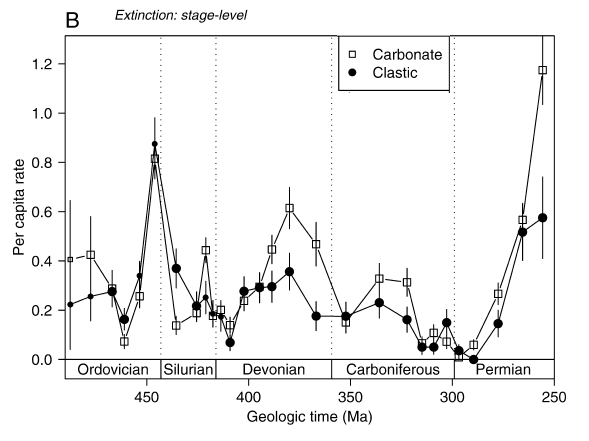
\includegraphics[height = 0.4\textheight, keepaspectratio = true]{figure/foote}
          
        \tiny{\attrib{Foote 2006 \textit{Paleobio.}}}
      \end{center}
    \end{column}
    \begin{column}{0.5\textwidth}
      \begin{itemize}
        \item carbonates, clastics, mixed
        \item lithology/deposition environment
        \item Pharenozoic decrease in carbonates:clastics
      \end{itemize}
    \end{column}
  \end{columns}
\end{frame}

\begin{frame}
  \frametitle{Habitat preference}

  \begin{columns}
    \begin{column}{0.5\textwidth}
      % image of habitat differences
      % predictions
    \end{column}
    \begin{column}{0.5\textwidth}
      \begin{itemize}
        \item on-shore, off-shore, none
        \item sea-level and energetics
        \item Pharenozoic decrease in on-shore:off-shore
      \end{itemize}
    \end{column}
  \end{columns}
\end{frame}

\begin{frame}
  \frametitle{Affixing strategy}

  \begin{columns}
    \begin{column}{0.5\textwidth}
      % image examples
      % predictions
    \end{column}
    \begin{column}{0.5\textwidth}
      \begin{itemize}
        \item pedunculate, reclining, cementing
        \item pedunculate:on-shore, reclining:off-shore
        \item environmental energetics
      \end{itemize}
    \end{column}
  \end{columns}
\end{frame}

\begin{frame}
  \frametitle{Assigning substrate and habitat}

  \begin{block}{Probability of assignment}
    \begin{align*}
      P(H_{1}|E) &= \frac{P(E|H_{1})P(H_{1})}{P(E|H_{1})P(H_{1}) + P(E|H_{2})P(H_{2})} \\
      P(E|H) &= \binom{n}{k} p^{k}(1 - p)^{n - k}
    \end{align*}

    \begin{itemize}
      \item \(n\): total \# of occ
      \item \(k\): \# (e.g.) carbonate occ
    \end{itemize}

    \tiny{\attrib{Simpson and Harnik 2009 \textit{Paleobiology}}}
  \end{block}
\end{frame}

\begin{frame}
  \frametitle{Models}
  % data source: PBDB (h/t Clapham)
  % substrate following Foote 2006 \textit{Paleobio.}
  % habitat following Kiesling et al. 2007 \textit{Proc. B}
  % traits: time--independent covariates
  % climate: ancillary time--dependent or Heaviside function
  % additive, interactive
  % exponential, Weibull, lognormal
\end{frame}

\begin{frame}
  \frametitle{Preliminary results: model comparison}

  % latex table generated in R 3.0.2 by xtable 1.7-1 package
% Thu Jan  9 14:42:10 2014
\begin{table}[ht]
\centering
\begin{tabular}{llrrrr}
 formula & distribution & shape & df & logLik & AICc \\ 
  \hline
\~{} aff & weibull & 1.91 & 4 & -497.5745 & 1003.4543 \\ 
  \~{} aff + hab & weibull & 1.92 & 6 & -496.8553 & 1006.3618 \\ 
  \~{} aff * hab & weibull & 1.94 & 10 & -495.7702 & 1013.3003 \\ 
  \~{} 1 & weibull & 1.76 & 2 & -515.1666 & 1034.4234 \\ 
  \~{} hab & weibull & 1.76 & 4 & -513.9591 & 1036.2236 \\ 
  \~{} aff & exponential &  & 3 & -532.8690 & 1071.9199 \\ 
  \~{} aff + hab & exponential &  & 5 & -532.5798 & 1075.6211 \\ 
  \~{} 1 & exponential &  & 1 & -540.9218 & 1083.8734 \\ 
  \~{} aff * hab & exponential &  & 9 & -532.3099 & 1084.0485 \\ 
  \~{} hab & exponential &  & 3 & -540.2811 & 1086.7439 \\ 
  \end{tabular}
\label{tab:brach}
\end{table}

\end{frame}

\begin{frame}
  \frametitle{Preliminary results: best substrate}

  \begin{center}
    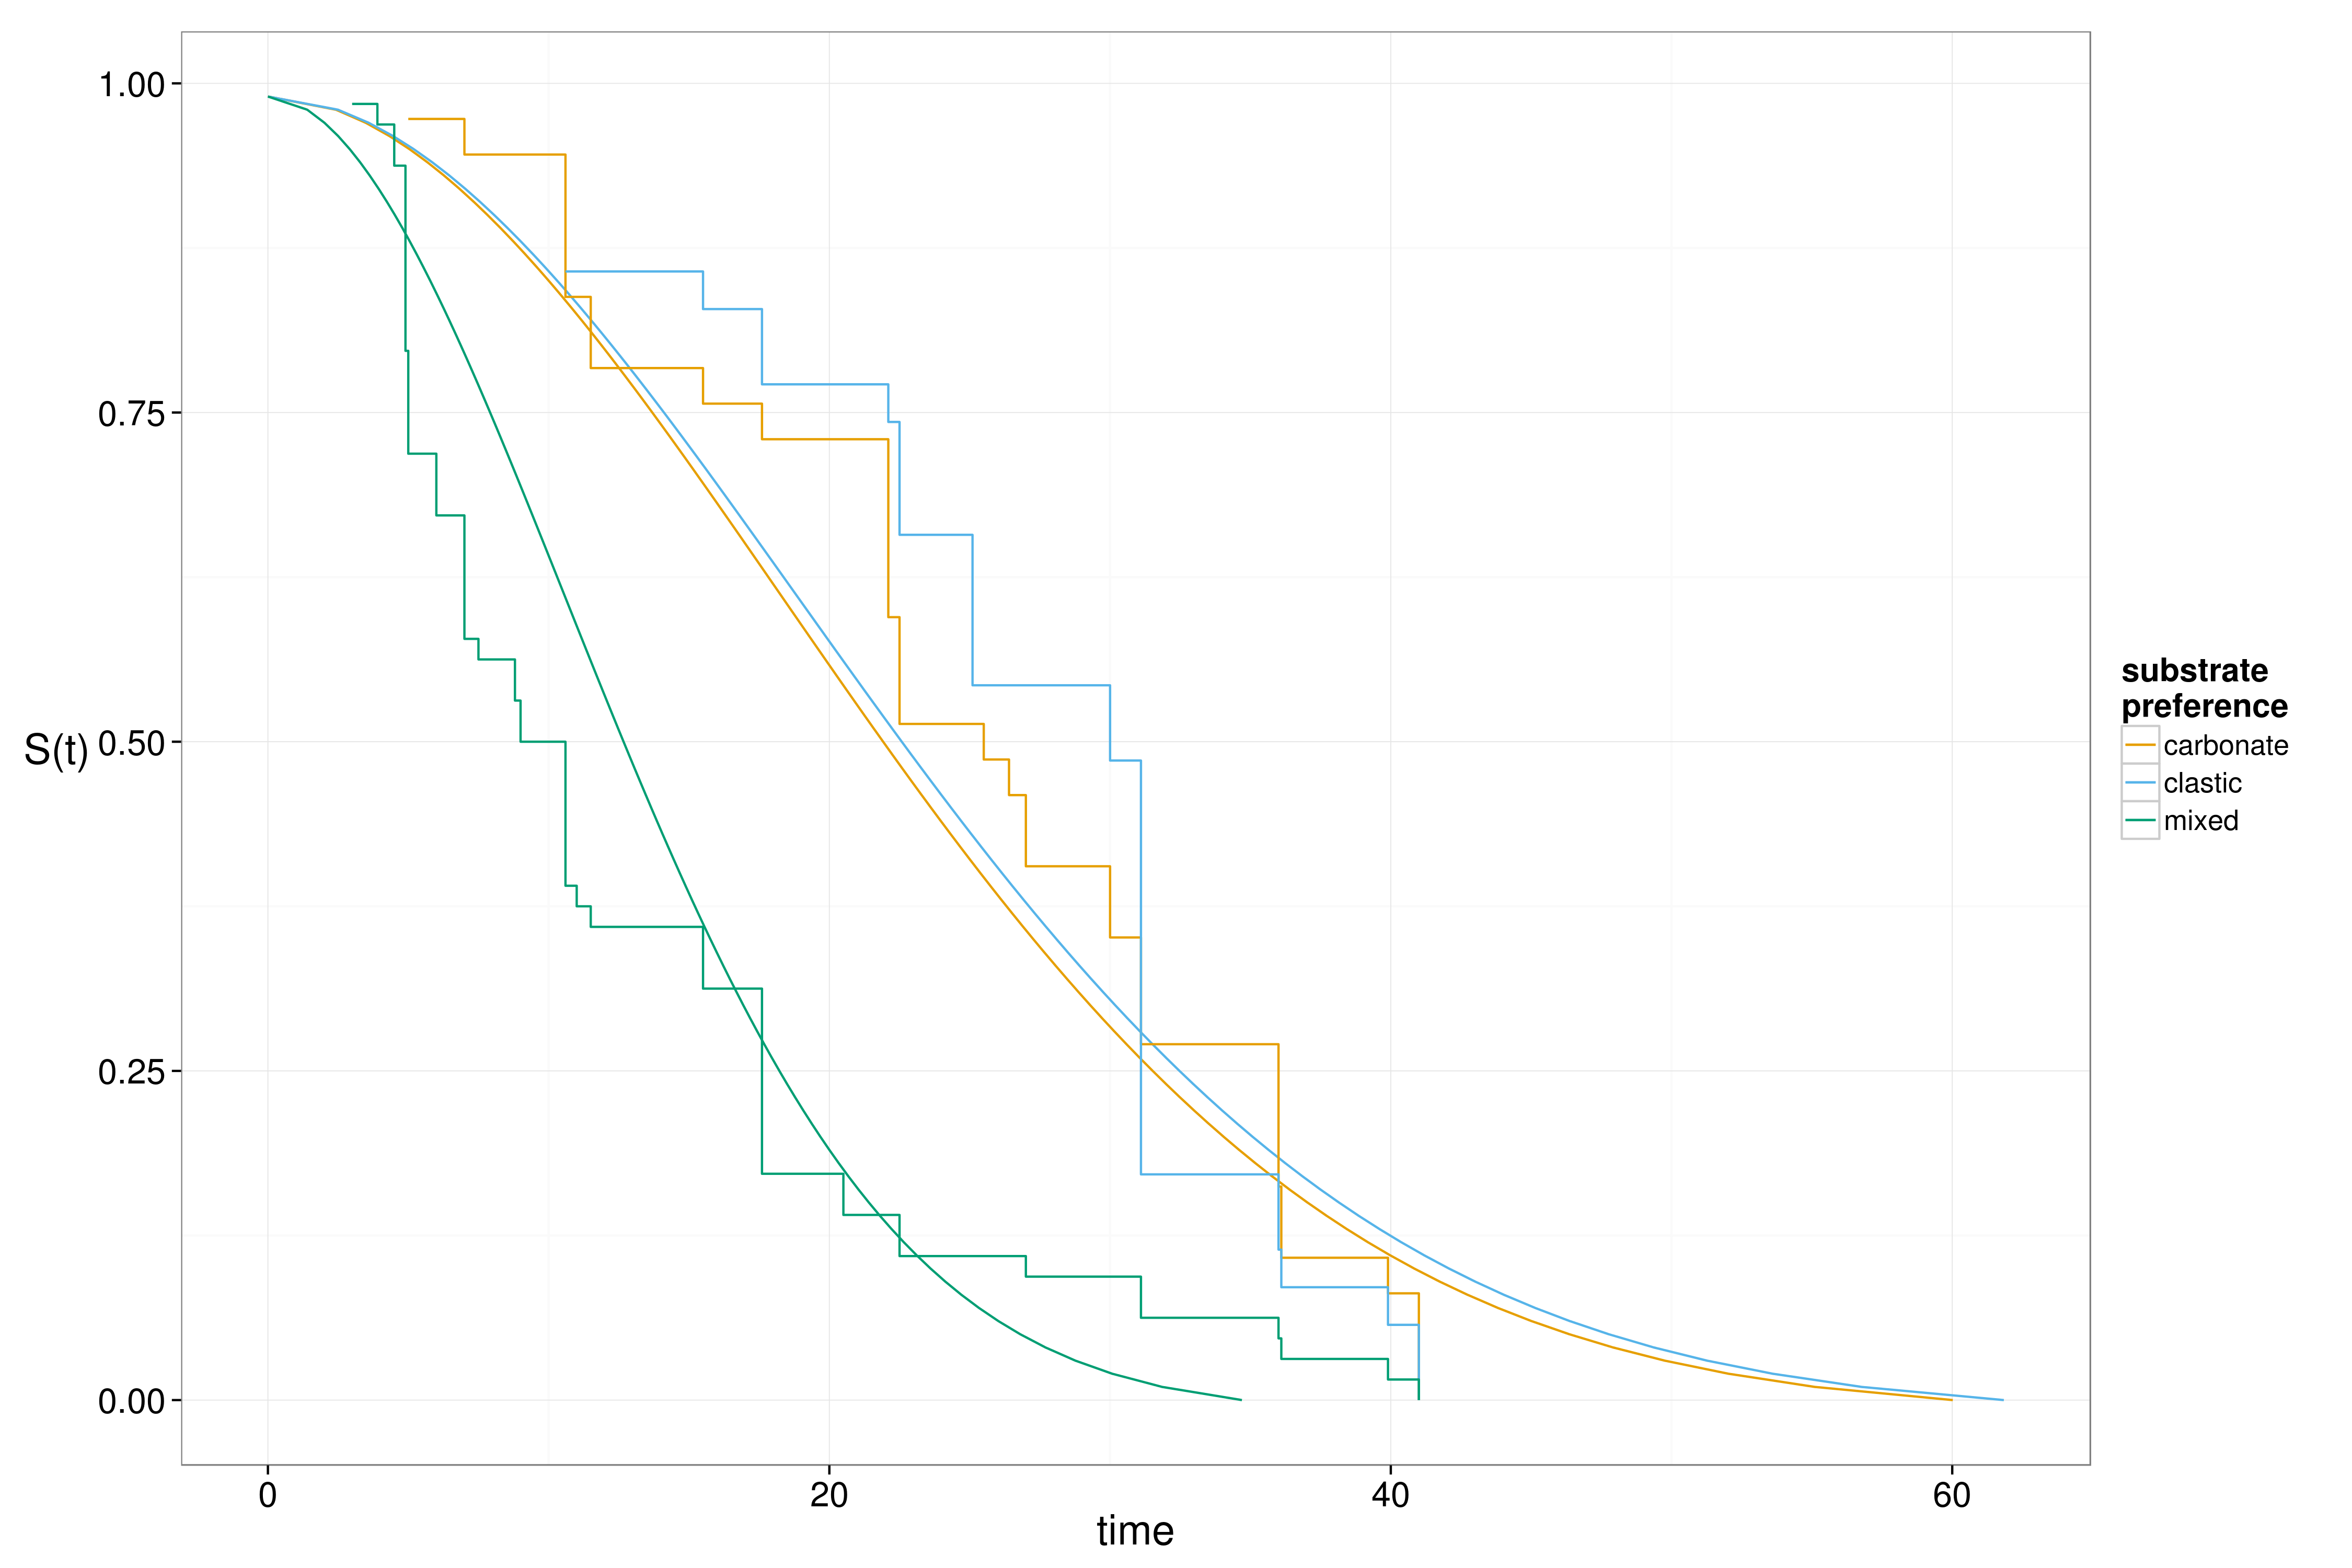
\includegraphics[height = 0.8\textheight, width = \textwidth, keepaspectratio = true]{figure/aff}
  \end{center}
\end{frame}

\begin{frame}
  \frametitle{Preliminary results: best habitat}

  \begin{center}
    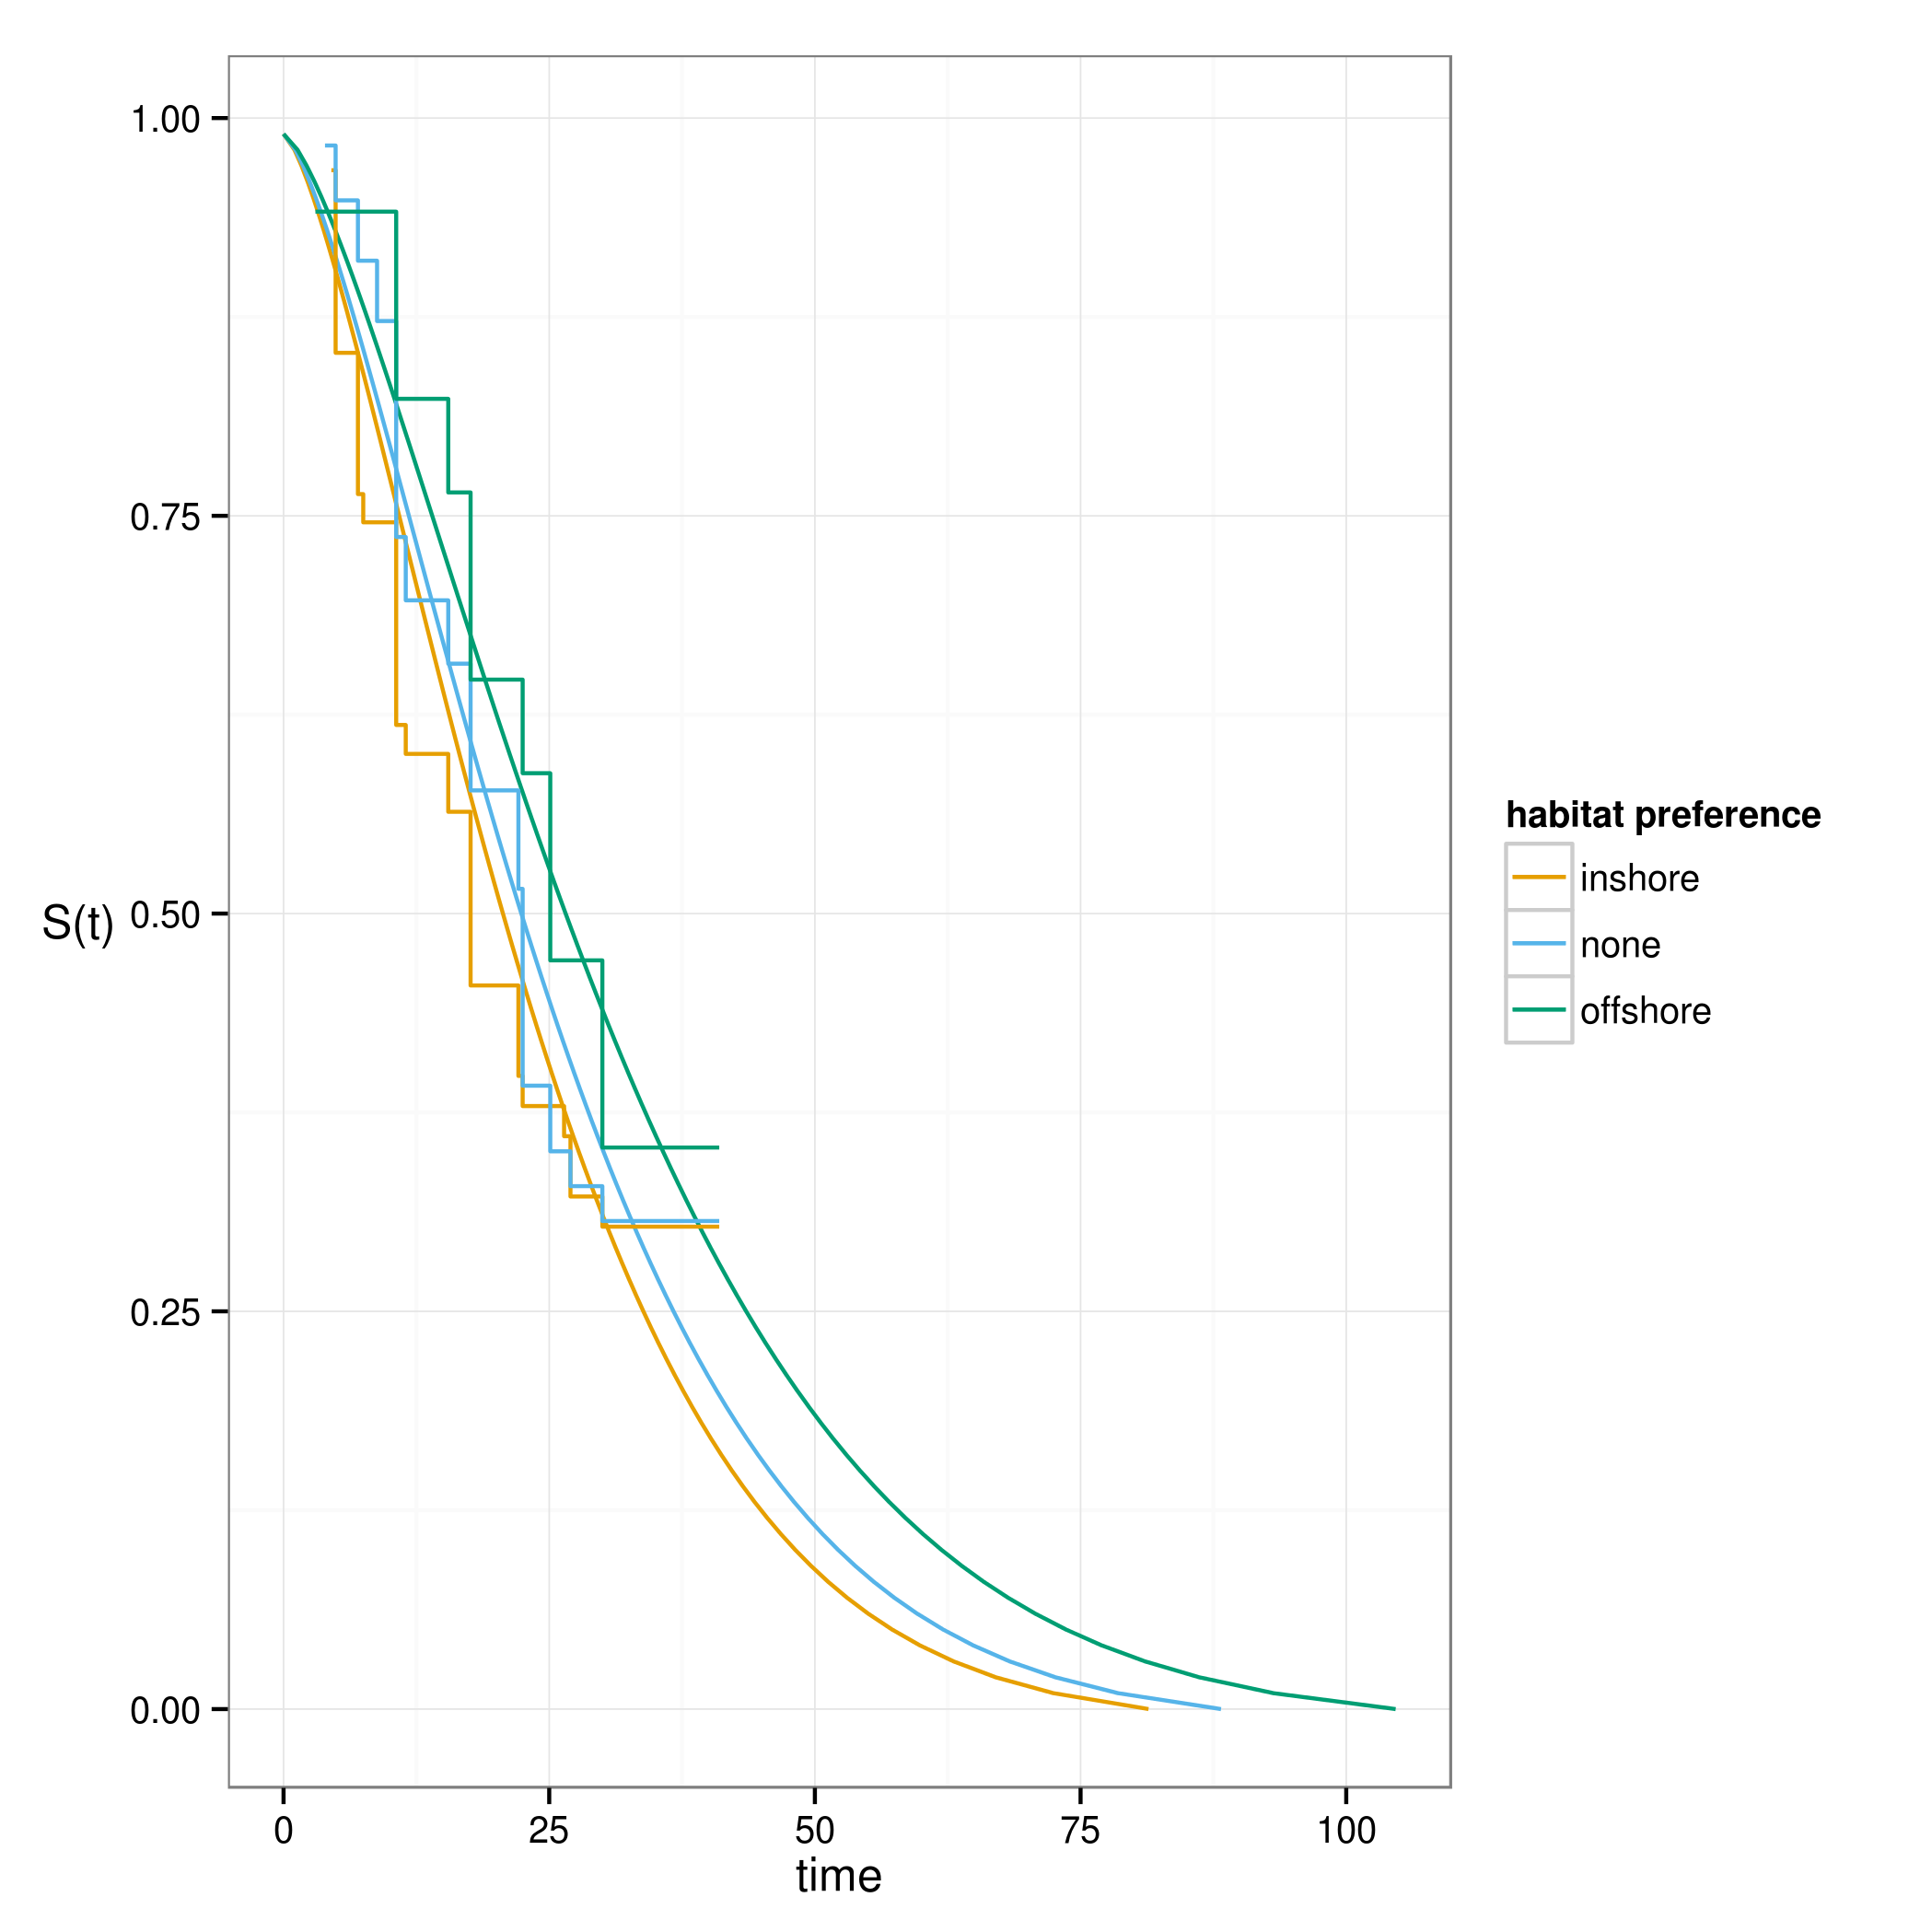
\includegraphics[height = 0.8\textheight, width = \textwidth, keepaspectratio = true]{figure/hab}
  \end{center}
\end{frame}


\section{Ecology and survival in Cenozoic mammals}

\begin{frame}
  \frametitle{Ecological traits}

  \begin{itemize}
    \item dietary category
      \begin{itemize}
        \item energetics
        \item availability
      \end{itemize}
    \item locomotor category
      \begin{itemize}
        \item availability
        \item dispersal
      \end{itemize}
    \item body size
      \begin{itemize}
        \item energetics
        \item home range size
      \end{itemize}
  \end{itemize}
\end{frame}

\begin{frame}
  \frametitle{Predictions: dietary category}
  \begin{columns}
    \begin{column}{0.5\textwidth}
      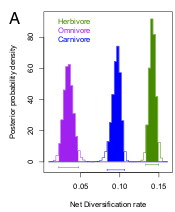
\includegraphics[height=0.8\textheight, width=\textwidth, keepaspectratio=true]{figure/dietdiv}

      \tiny{\attrib{Price \textit{et al.} 2012 \textit{PNAS}}}
      % probably want an additional image
    \end{column}
    \begin{column}{0.5\textwidth}
      \begin{itemize}
        \item trophic hierarchy \\(stability \(\to\) duration)
          \begin{itemize}
            \item herb: most stable, longest duration
            \item carni: least stable, shortest duration
            \item omni: avg. stability, avg. duration
          \end{itemize}
        \item \(\uparrow\) diversification
          \begin{itemize}
            \item \(\uparrow\) origination; \(\simeq\) extinction
            \item \(\simeq\) origination; \(\downarrow\) extinction
          \end{itemize}
      \end{itemize}
    \end{column}
  \end{columns}
\end{frame}

\begin{frame}
  \frametitle{Predictions: locomotor category}
  
  \begin{columns}
    \begin{column}{0.5\textwidth}
      % image from a Janis paper?
      % look in Blois2009 for ideas
    \end{column}
    \begin{column}{0.5\textwidth}
      \begin{itemize}
        \item Paleogene \(\to\) Neogene
          \begin{itemize}
            \item open \(\to\) closed environment
          \end{itemize}
      \end{itemize}
    \end{column}
  \end{columns}
\end{frame}

\begin{frame}
  \frametitle{Predictions: body size}

  \begin{columns}
    \begin{column}{0.5\textwidth}
      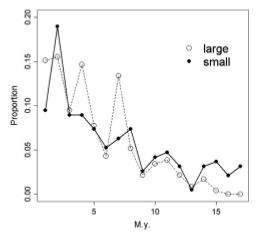
\includegraphics[height=0.4\textheight, width=\textwidth, keepaspectratio=true]{figure/liowmam}

      \tiny{\attrib{Liow \textit{et al.} 2008 \textit{PNAS}}}

      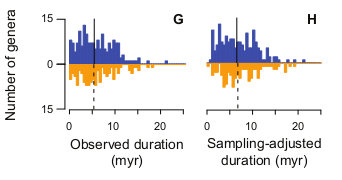
\includegraphics[height=0.4\textheight, width=\textwidth, keepaspectratio=true]{figure/susumu}

      \tiny{\attrib{Tomiya 2013 \textit{Am. Nat.}}}
    \end{column}
    \begin{column}{0.5\textwidth}
      \begin{itemize}
        \item \(\uparrow\) body size, \(\uparrow\) energy req, \\\(\uparrow\) range size, \(\downarrow\) extinction
        \item Europe
          \begin{itemize}
            \item lrg body size genera: \\\(\uparrow\) extinction
          \end{itemize}
        \item North America
          \begin{itemize}
            \item generic body size: \\\(\simeq\) extinction
          \end{itemize}
      \end{itemize}
    \end{column}
  \end{columns}
\end{frame}

\begin{frame}
  \frametitle{Methodology}
  % genus versus species
  % exponential, Weibull, lognormal
  % time--independent: alone, additive, interactive
  % ancillary time--dependent: Zachos curve
  % Paleogene versus Neogene
  % data source: PBDB, NOW, museum collections, published compliations
  %   h/t Alroy
\end{frame}


\begin{frame} % consider cutting this or moving to ``Appendix''
  \frametitle{Biases to survival: a simulation study}

  \begin{columns}
    \begin{column}{0.5\textwidth}
      %image of a bunch of random trees?
    \end{column}
    \begin{column}{0.5\textwidth}
      \begin{itemize}
        \item bias away from \(h(t) = \lambda\)
          \begin{itemize}
            \item species:genus
            \item anagenesis/cryptic speciation
          \end{itemize}
        \item time-homogeneous birth-death model
          \begin{itemize}
            \item common phylogenetic model
            \item constant \(p\), \(b\)
            \item expected \(S(t) = \exp^{-\lambda t}\)
            \item vary (cryptic) anagenesis
          \end{itemize}
      \end{itemize}
    \end{column}
  \end{columns}
\end{frame}


\section{Community connectedness in Cenozoic mammals}

\begin{frame}
  \frametitle{Community connectedness}
  \begin{definition}
    The degree to which localities are composed of endemic versus cosmopolitan taxa, and how similar this ratio is across localities.
  \end{definition}
  % figures from Sidor et al 2013?
\end{frame}

\begin{frame}
  \frametitle{Biogeographic networks}
  \begin{columns}
    \begin{column}{0.5\textwidth}
      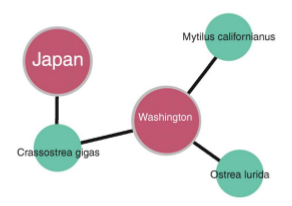
\includegraphics[height = 0.8\textheight, width = \textwidth, keepaspectratio = true]{figure/vilhena}

      \tiny{\attrib{Vilhena \textit{et al.} 2013 \textit{Sci. Reports}}}
    \end{column}
    \begin{column}{0.5\textwidth}
      \begin{itemize}
        \item taxa: species
        \item locality: 2x2 equal--area map projection grid
        \item 2 My intervals
        \item PBDB, NOW, \\museum collections, compilations
      \end{itemize}
    \end{column}
  \end{columns}
\end{frame}

\begin{frame}
  \frametitle{Average relative number of endemics}

  \begin{columns}
    \begin{column}{0.5\textwidth}
      % pictures
    \end{column}
    \begin{column}{0.5\textwidth}
      \[
        E = \frac{\sum_{i = 1}^{L} \frac{u_{i}}{n_{i}}}{L}
      \]

      \begin{itemize}
        \item \(L\): number of localities
        \item \(u\): number of taxa unique to a locality
        \item \(n\): number of taxa at a locality
        \item \(0 \leq E \leq 1\)
      \end{itemize}
    \end{column}
  \end{columns}
\end{frame}

\begin{frame}
  \frametitle{Average relative occupancy per taxon}

  \begin{columns}
    \begin{column}{0.5\textwidth}
      % pictures
    \end{column}
    \begin{column}{0.5\textwidth}
      \[
        Occ = \frac{\sum_{i = 1}^{N} \frac{l_{i}}{L}}{N}
      \]

      \begin{itemize}
        \item \(N\): total number of taxa
        \item \(l\): number of localities a taxon occurs at
        \item \(L\): number of localities
        \item \(0 \leq Occ \leq 1\)
      \end{itemize}
    \end{column}
  \end{columns}
\end{frame}

\begin{frame}
  \frametitle{Biogeographic connectedness}

  \begin{columns}
    \begin{column}{0.5\textwidth}
      \begin{center}
        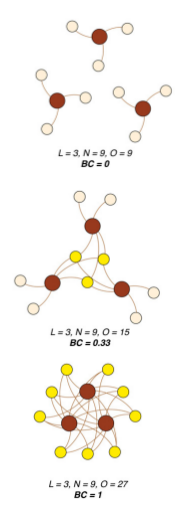
\includegraphics[height=0.8\textheight,width=\textwidth,keepaspectratio=true]{figure/bc}

        \tiny{\attrib{Sidor et al. 2013 \textit{PNAS}}}
      \end{center}
    \end{column}
    \begin{column}{0.5\textwidth}
      \[
        BC = \frac{O - N}{LN - N}
      \]

      \begin{itemize}
        \item \(O\): number of occurrences
        \item \(N\): total number of taxa
        \item \(L\): number of localities
        \item \(0 \leq BC \leq 1\)
      \end{itemize}
    \end{column}
  \end{columns}
\end{frame}

\begin{frame}
  \frametitle{Code length}
  \begin{center}
    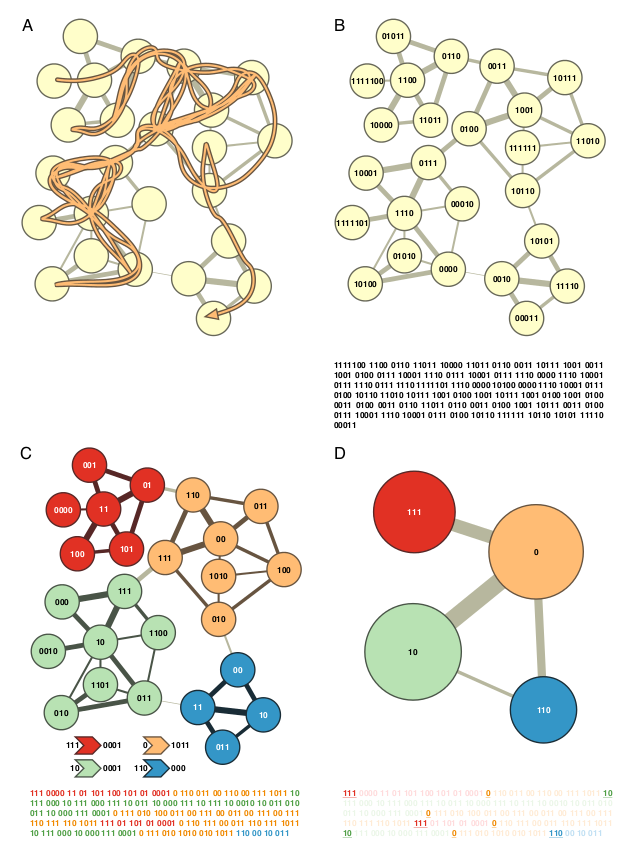
\includegraphics[height=0.8\textheight,width=\textwidth,keepaspectratio=true]{figure/map}

    \tiny{\attrib{Rosvall and Bergstrom 2008 \textit{PNAS}}}
  \end{center}

  % break up by each section so it is easier to explain?
\end{frame}

\begin{frame}
  \frametitle{Global versus regional versus local scale processes}

  \begin{columns}
    \begin{column}{0.55\textwidth}
      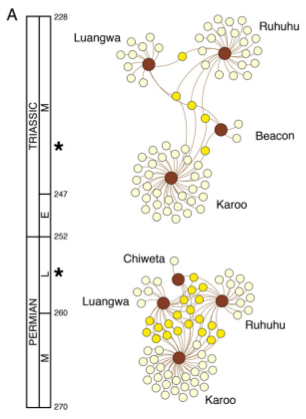
\includegraphics[height=0.7\textheight,width=\textwidth,keepaspectratio=true]{figure/permian}

      \tiny{\attrib{Sidor et al. 2013 \textit{PNAS}}}
    \end{column}
    \begin{column}{0.45\textwidth}
      \begin{itemize}
        \item global
          \begin{itemize}
            \item corr w/ global climate
            \item multiple regions corr
          \end{itemize}
        \item regional
          \begin{itemize}
            \item \(\downarrow E\), \(\uparrow Occ\), \\\(\uparrow BC\), \(\uparrow\) code
          \end{itemize}
        \item local
          \begin{itemize}
            \item \(\uparrow E\), \(\downarrow Occ\), \\\(\downarrow BC\), \(\downarrow\) code
          \end{itemize}
        \item \alert{not mutually exclusive}
      \end{itemize}
    \end{column}
  \end{columns}
\end{frame}

\begin{frame}
  \frametitle{Expectations: locomotor category}

  \begin{columns}
    \begin{column}{0.6\textwidth}
      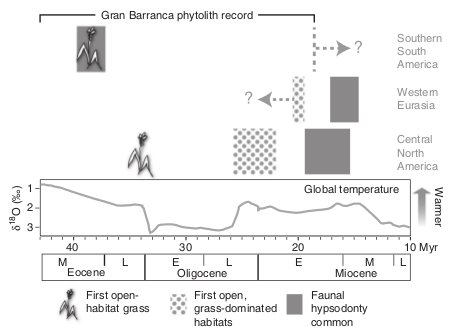
\includegraphics[height=0.8\textheight,width=\textwidth,keepaspectratio=true]{figure/stromberg}

      \tiny{\attrib{Str\"{o}mberg \textit{et al.} 2013 \textit{Nature Com.}}}
    \end{column}
    \begin{column}{0.4\textwidth}
      \begin{itemize}
        \item arboreal
          \begin{itemize}
            \item \(\uparrow E\), \(\uparrow\) code
            \item \(\downarrow BC\), \(\downarrow Occ\)
          \end{itemize}
        \item ground dwelling
          \begin{itemize}
            \item \(\downarrow E\), \(\downarrow\) code
            \item \(\uparrow BC\), \(\uparrow Occ\)
          \end{itemize}
        \item scansorial
          \begin{itemize}
            \item constant \(\lor\) random
          \end{itemize}
      \end{itemize}
    \end{column}
  \end{columns}
\end{frame}

\begin{frame}
  \frametitle{Expectations: dietary category}

  \begin{columns}
    \begin{column}{0.6\textwidth}
      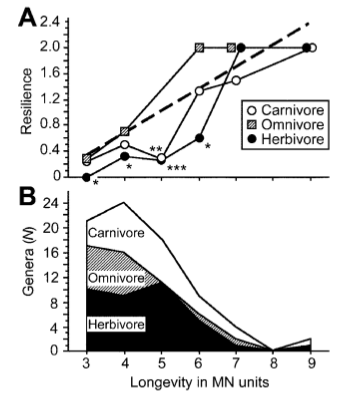
\includegraphics[height=0.7\textheight,width=\textwidth,keepaspectratio=true]{figure/jernvall}

      \tiny{\attrib{Jernvall and Fortelius 2004 \textit{Am. Nat.}}}
    \end{column}
    \begin{column}{0.4\textwidth}
      \begin{itemize}
        \item herbivore
          \begin{itemize}
            \item most like all taxa
          \end{itemize}
        \item carnivore
          \begin{itemize}
            \item constant \(\lor\) corr w/ herbivores
          \end{itemize}
        \item omnivore
          \begin{itemize}
            \item constant \(\lor\) random
          \end{itemize}
      \end{itemize}
    \end{column}
  \end{columns}
\end{frame}

\begin{frame}
  \frametitle{Community connectedness of North America}
\end{frame}

\begin{frame}
  \frametitle{Community connectedness of Europe}
\end{frame}

\begin{frame}
  \frametitle{Community connectedness of South America}
\end{frame}

% include phylogenetic similarity in ``Appendix''?

\begin{frame}
  \frametitle{Preliminary results: NA, Eur}

  \begin{center}
    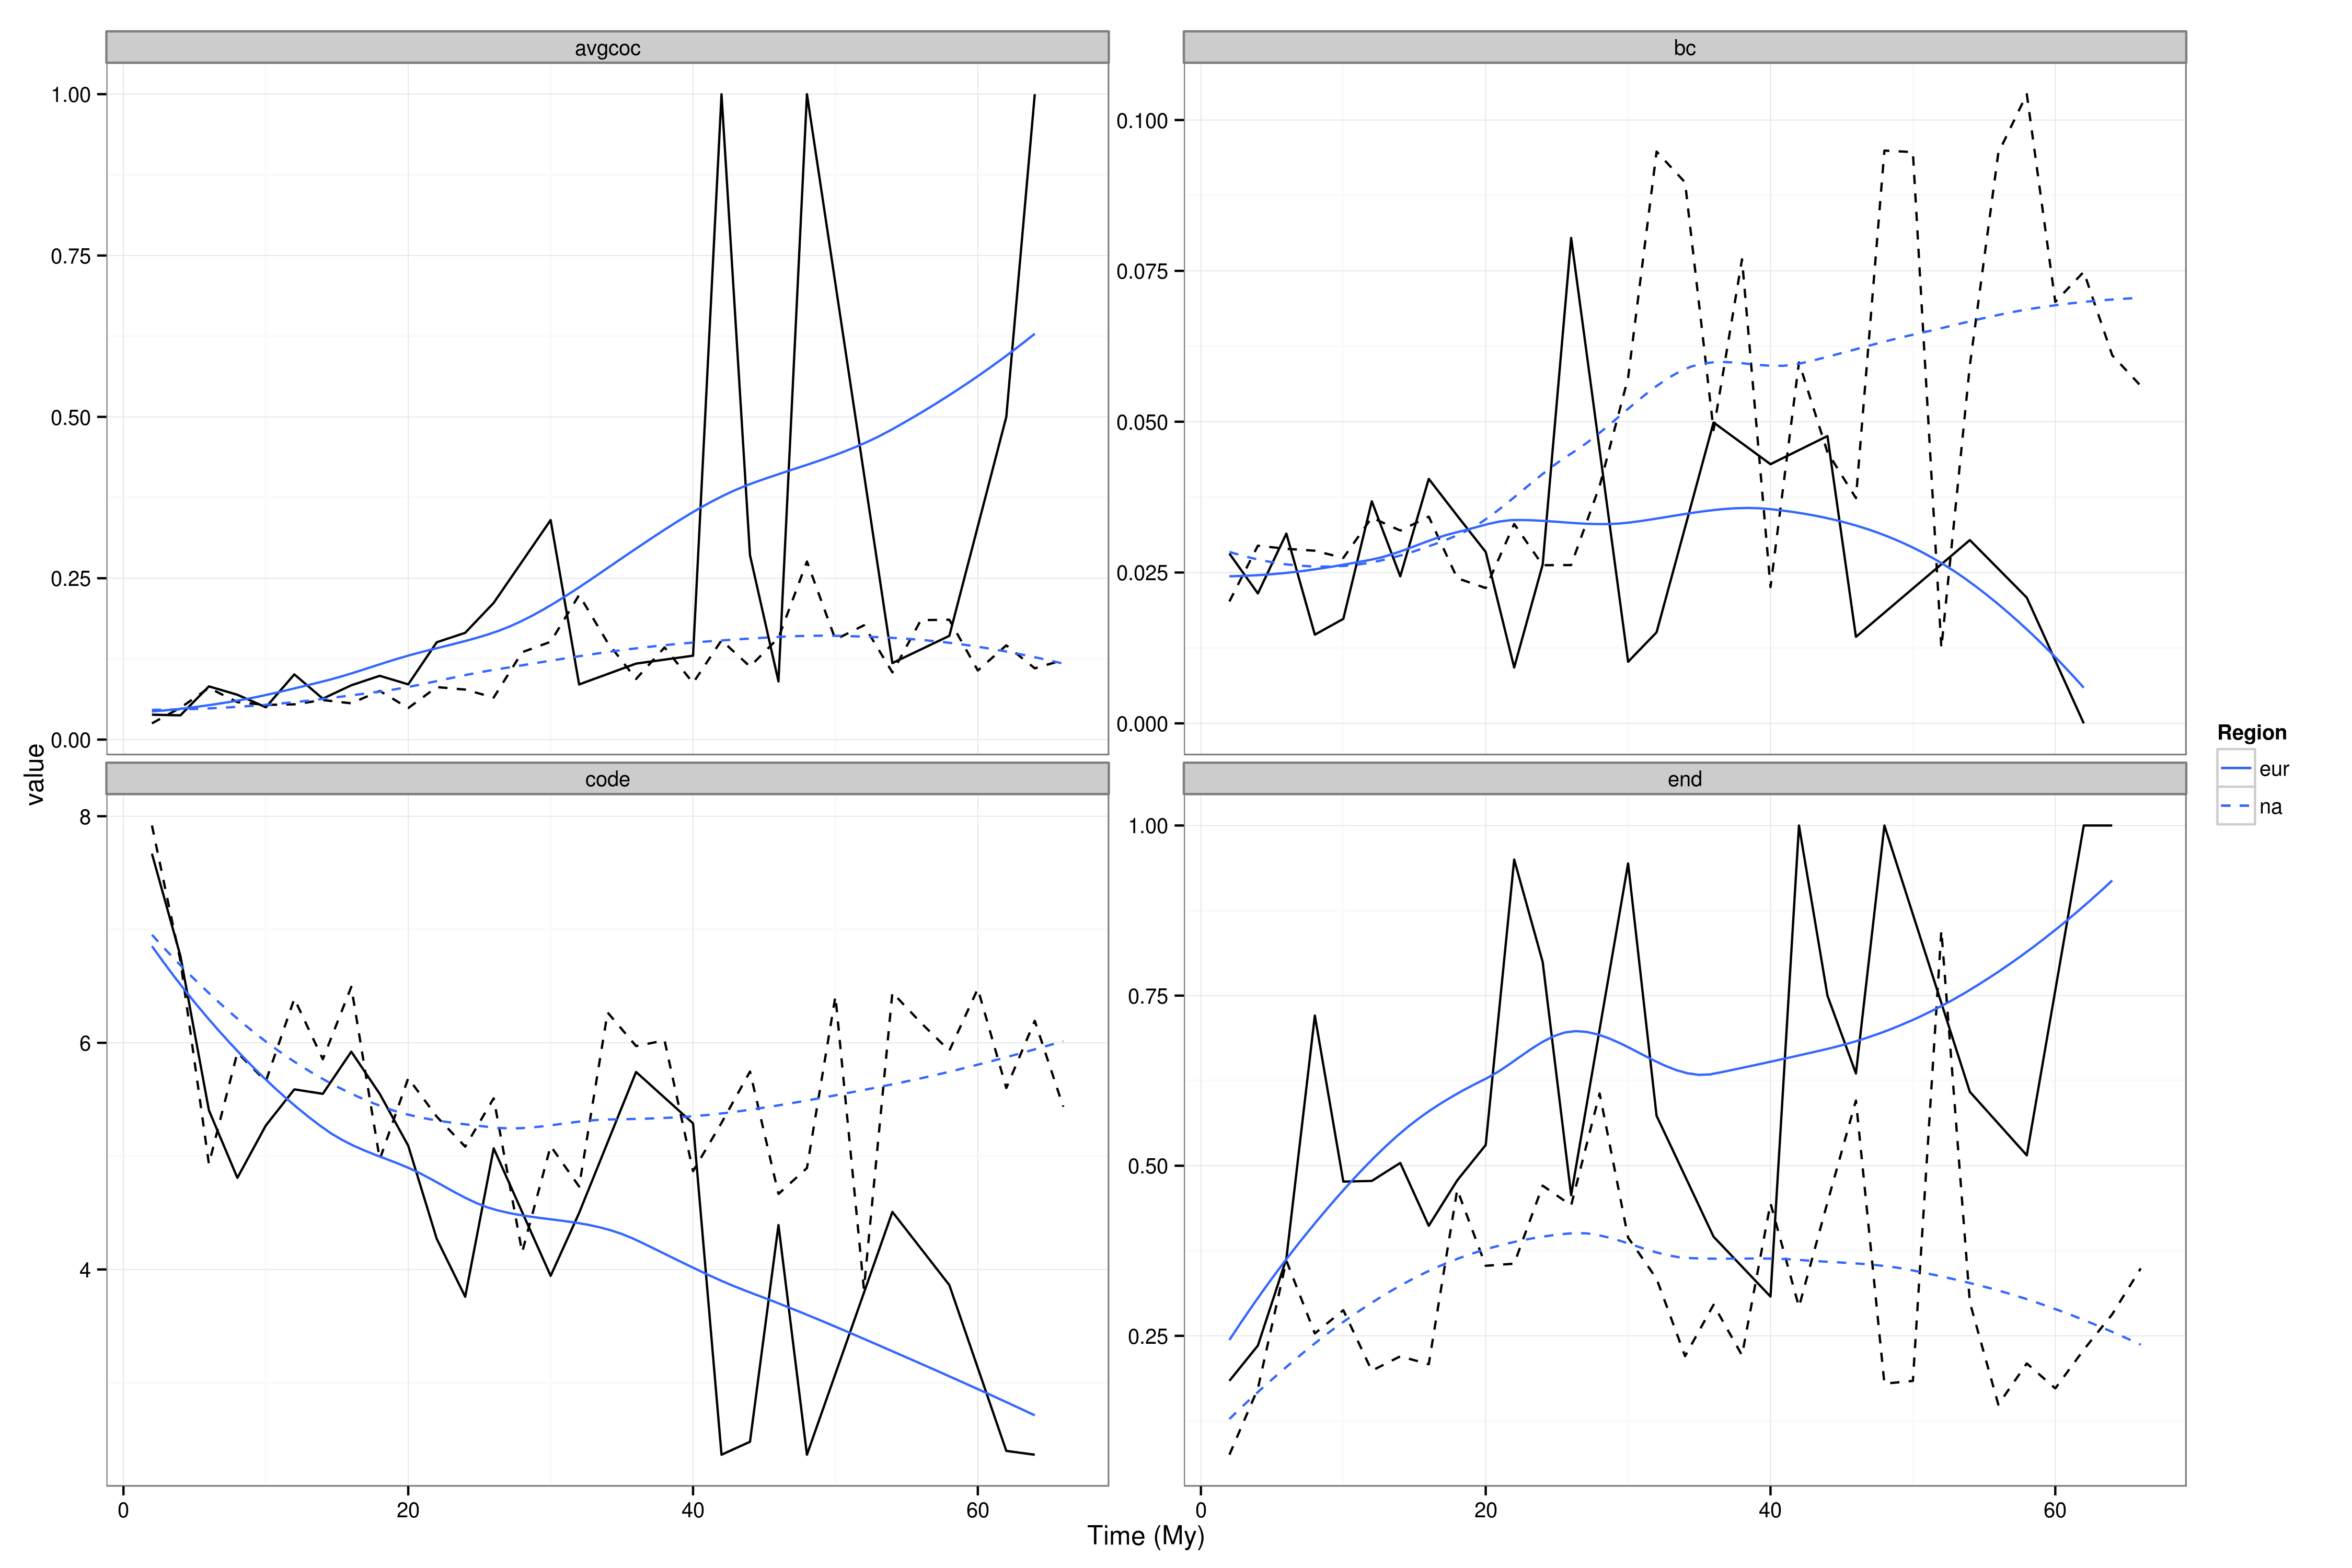
\includegraphics[height = 0.8\textheight, width = \textwidth, keepaspectratio = true]{figure/gen_bin}
  \end{center}
\end{frame}

\begin{frame}
  \frametitle{Preliminary results: locomotor category}

  \tiny{North America}
  \begin{center}
    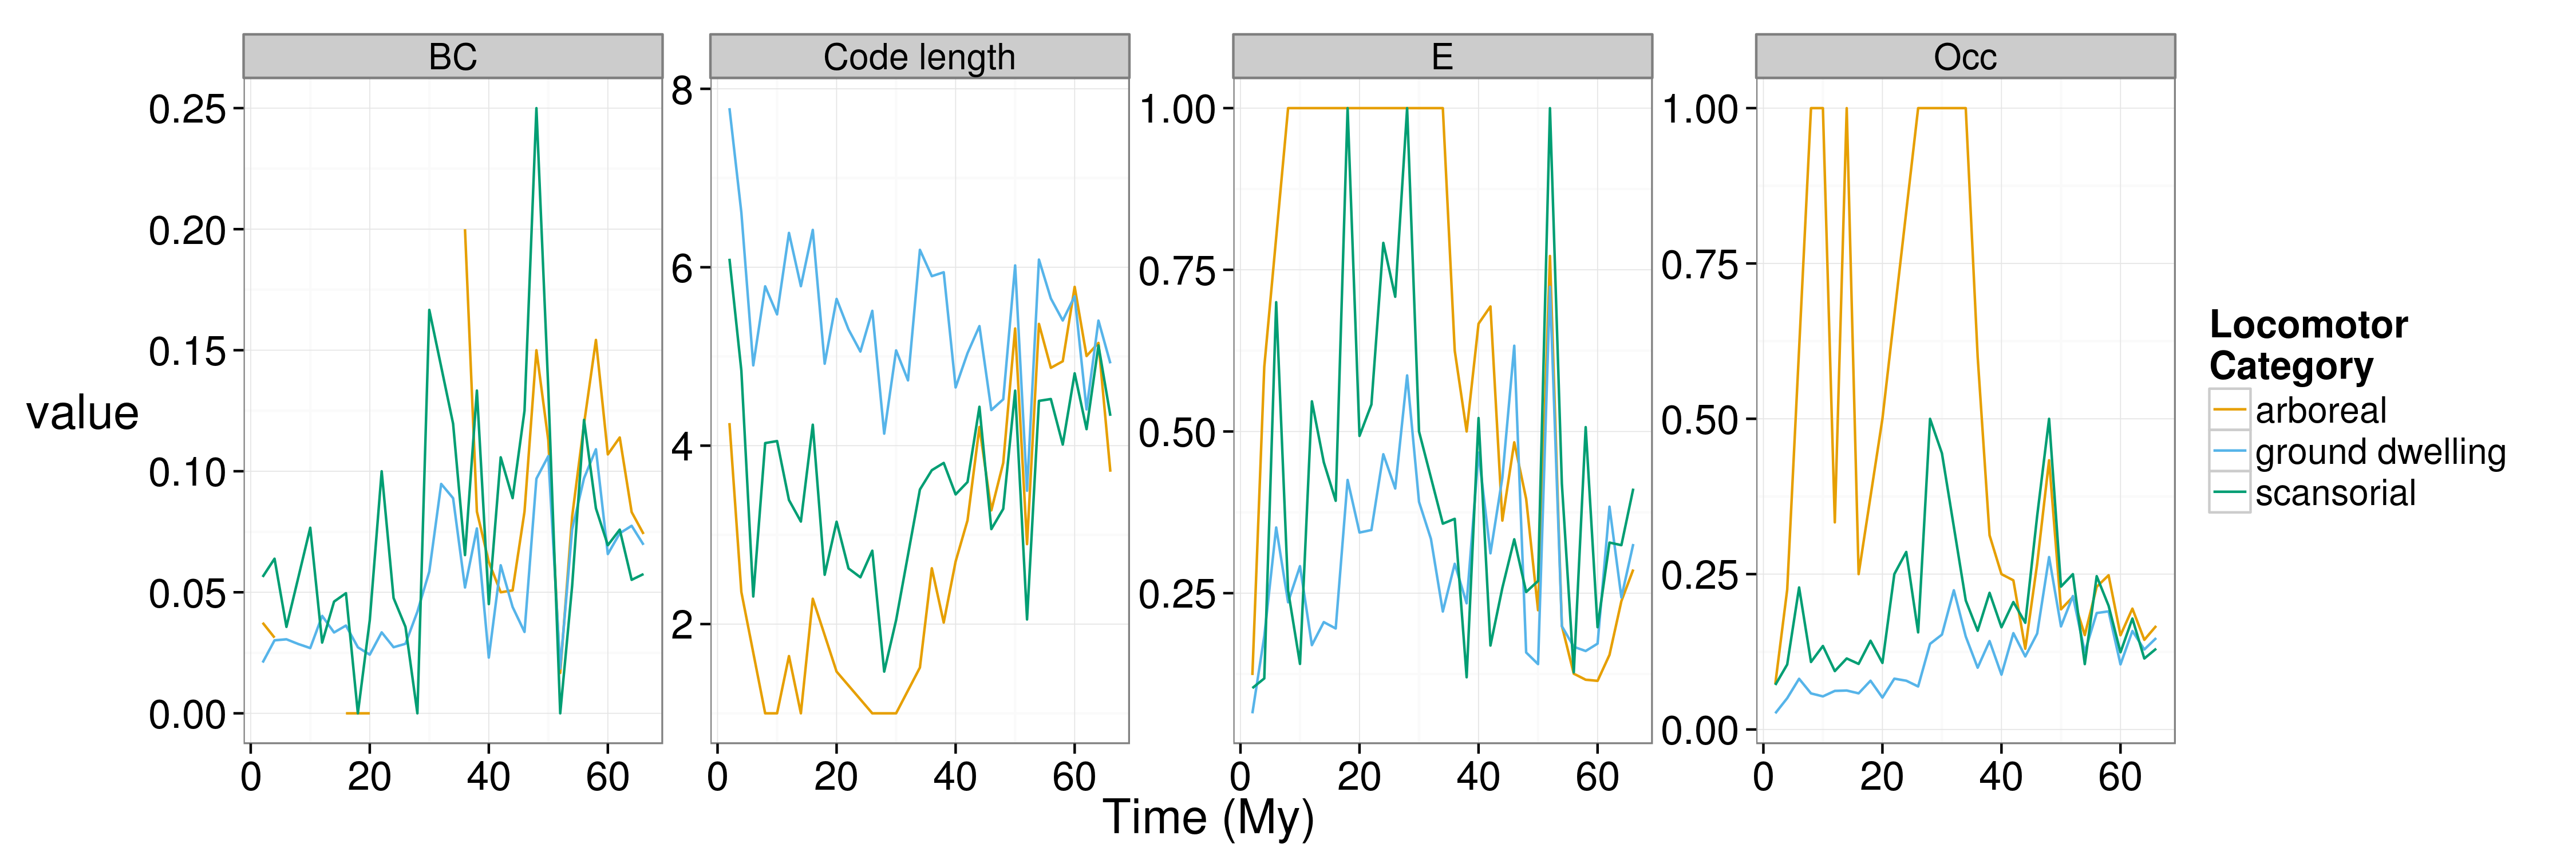
\includegraphics[height = 0.35\textheight, width = \textwidth, keepaspectratio = true]{figure/na_lf}
  \end{center}

  \tiny{Europe}
  \begin{center}
    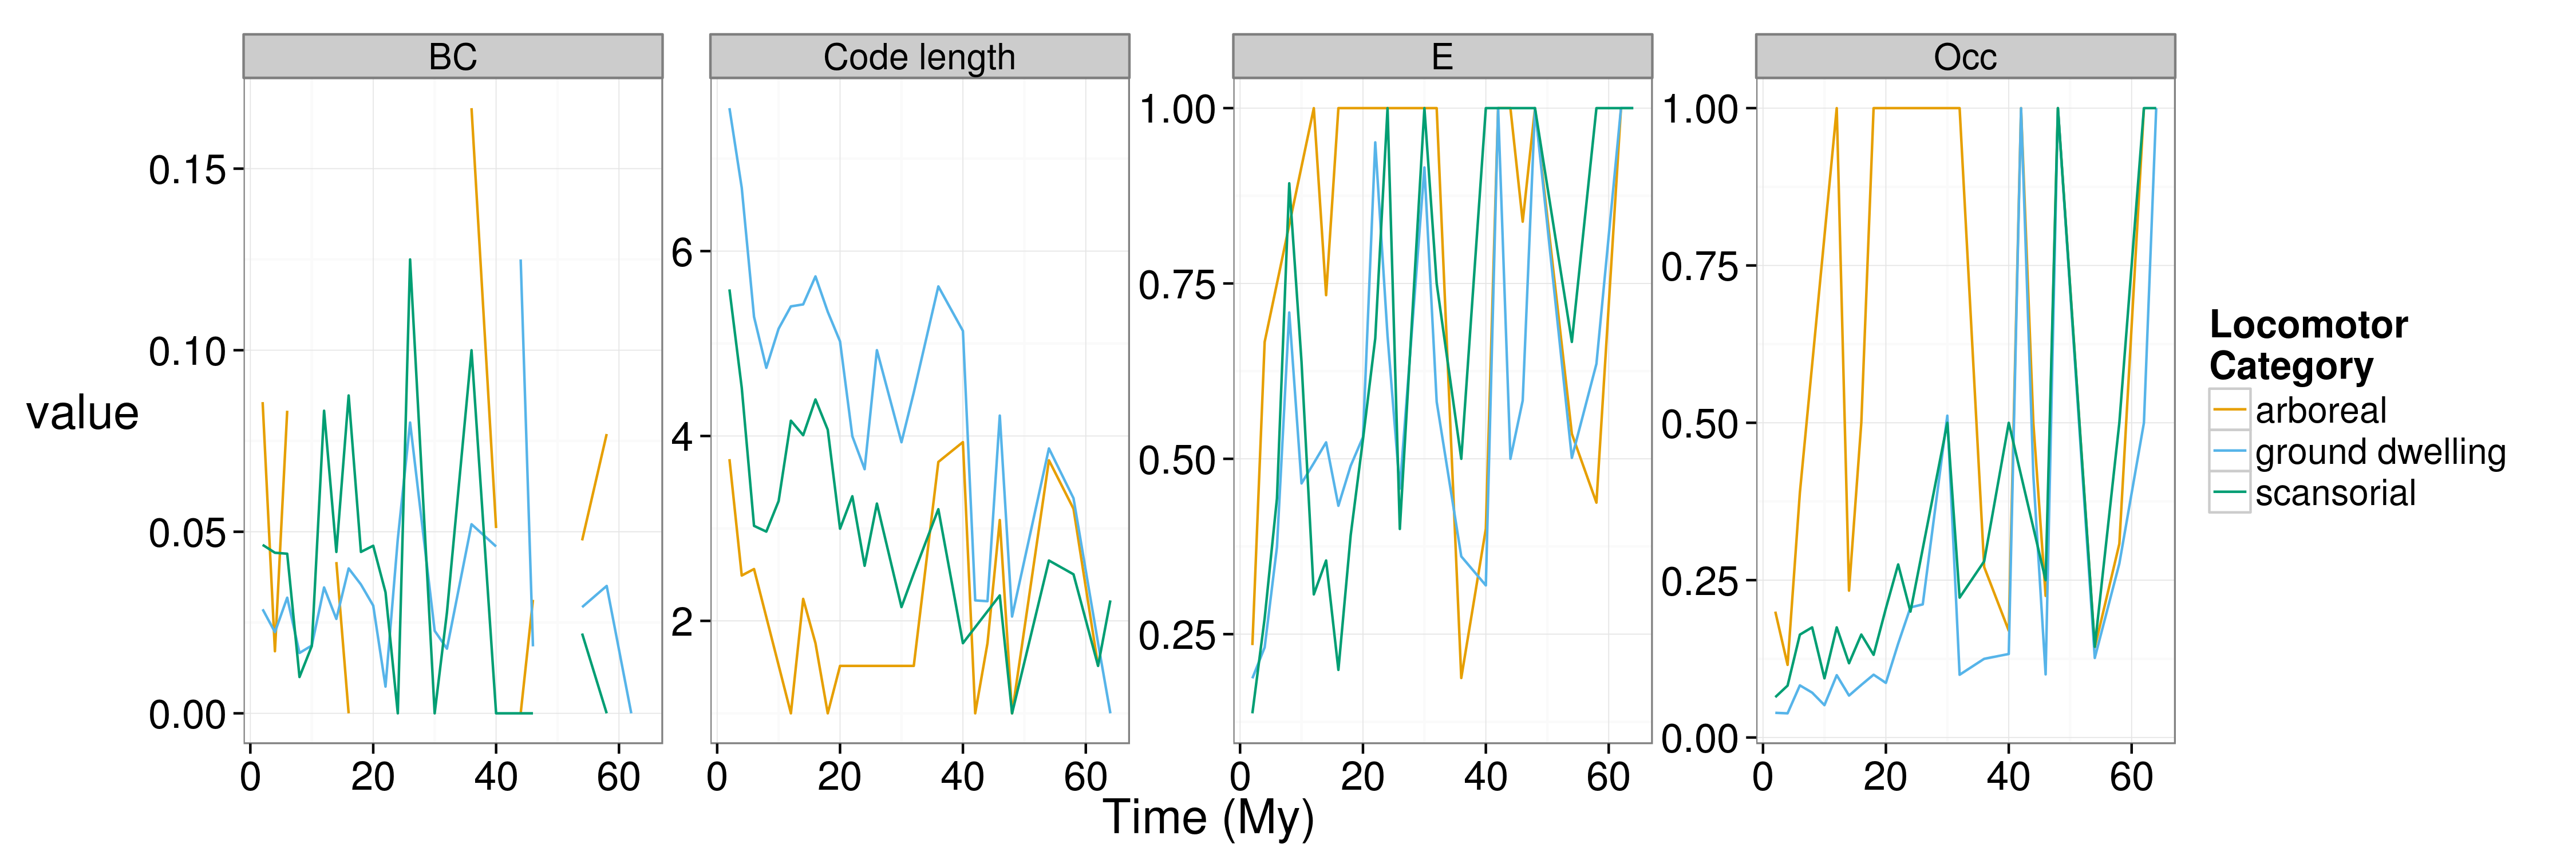
\includegraphics[height = 0.35\textheight, width = \textwidth, keepaspectratio = true]{figure/er_lf}
  \end{center}
\end{frame}

\begin{frame}
  \frametitle{Preliminary results: dietary category}

  \tiny{North America}
  \begin{center}
    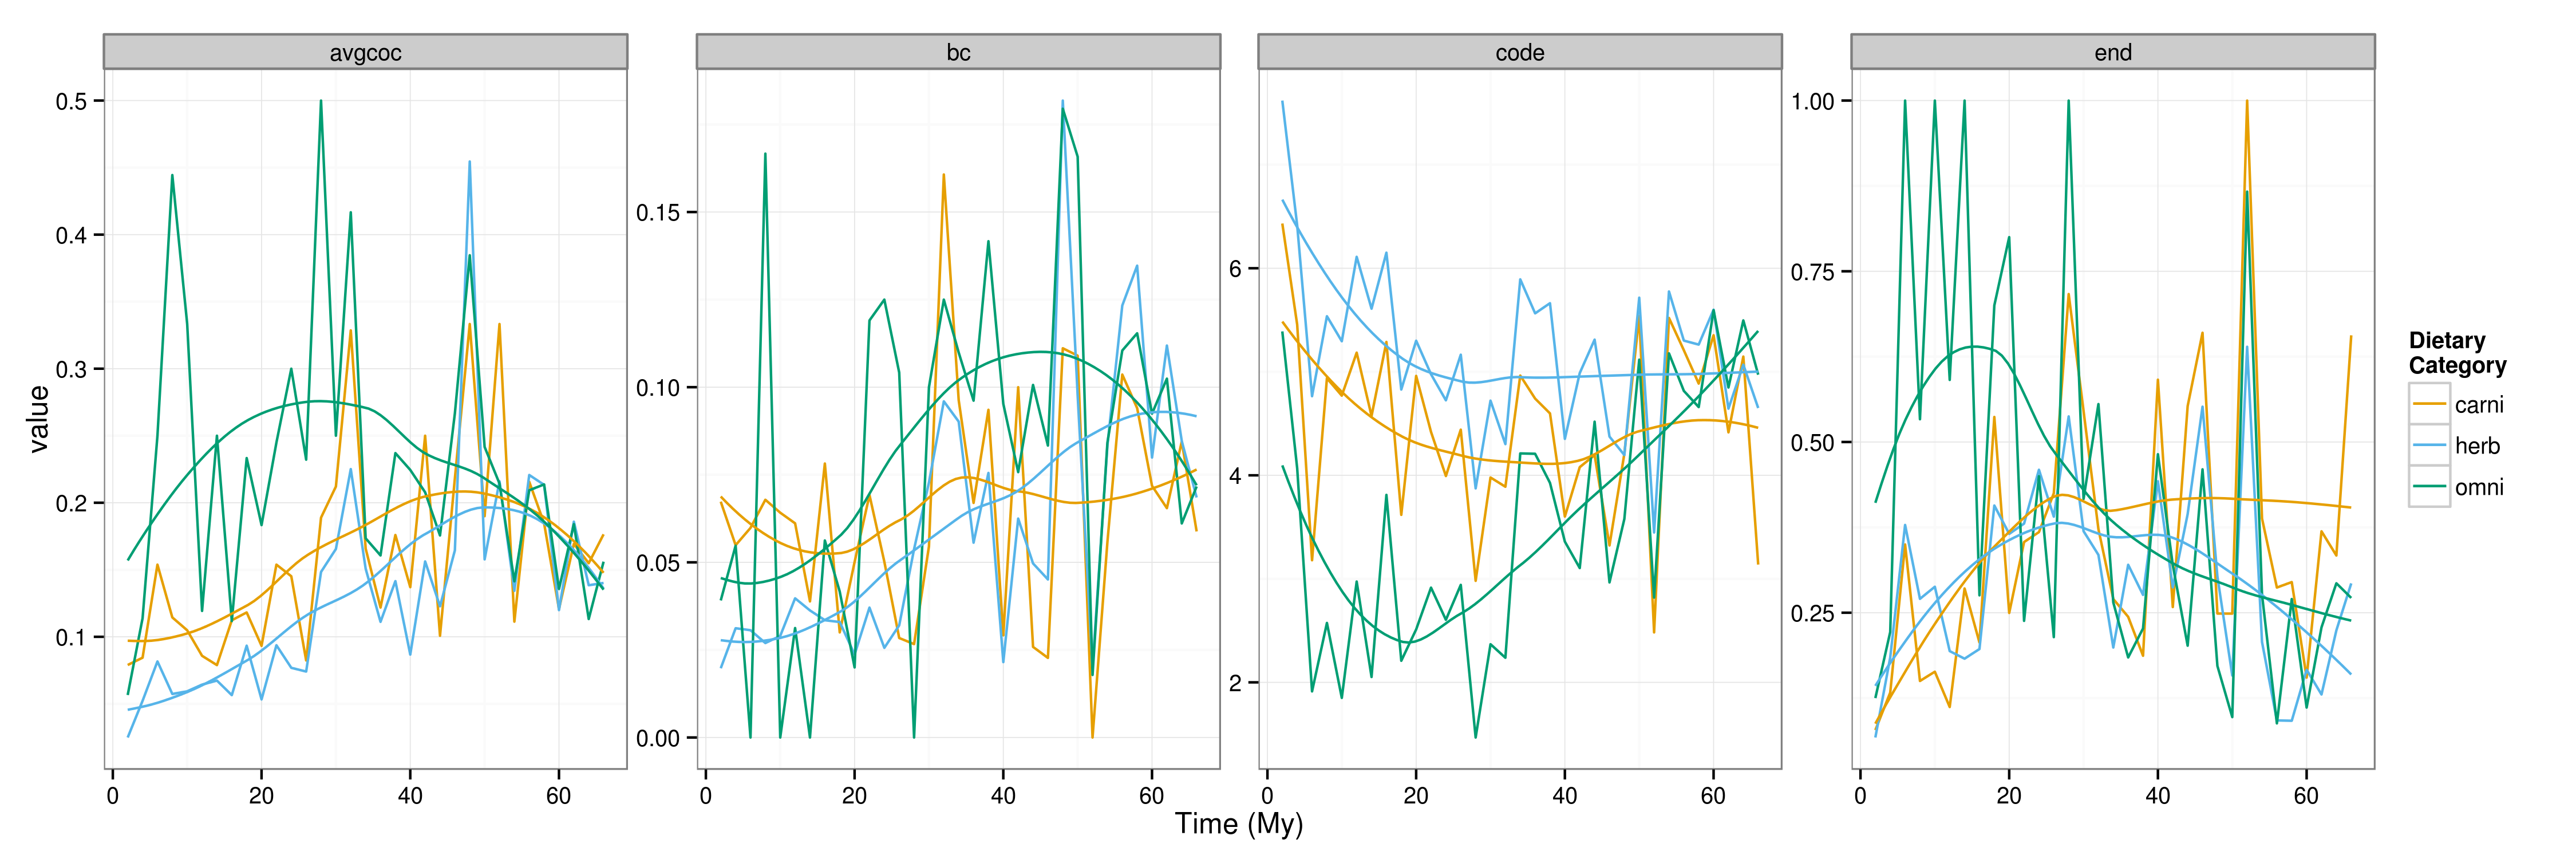
\includegraphics[height = 0.35\textheight, width = \textwidth, keepaspectratio = true]{figure/na_dt}
  \end{center}

  \tiny{Europe}
  \begin{center}
    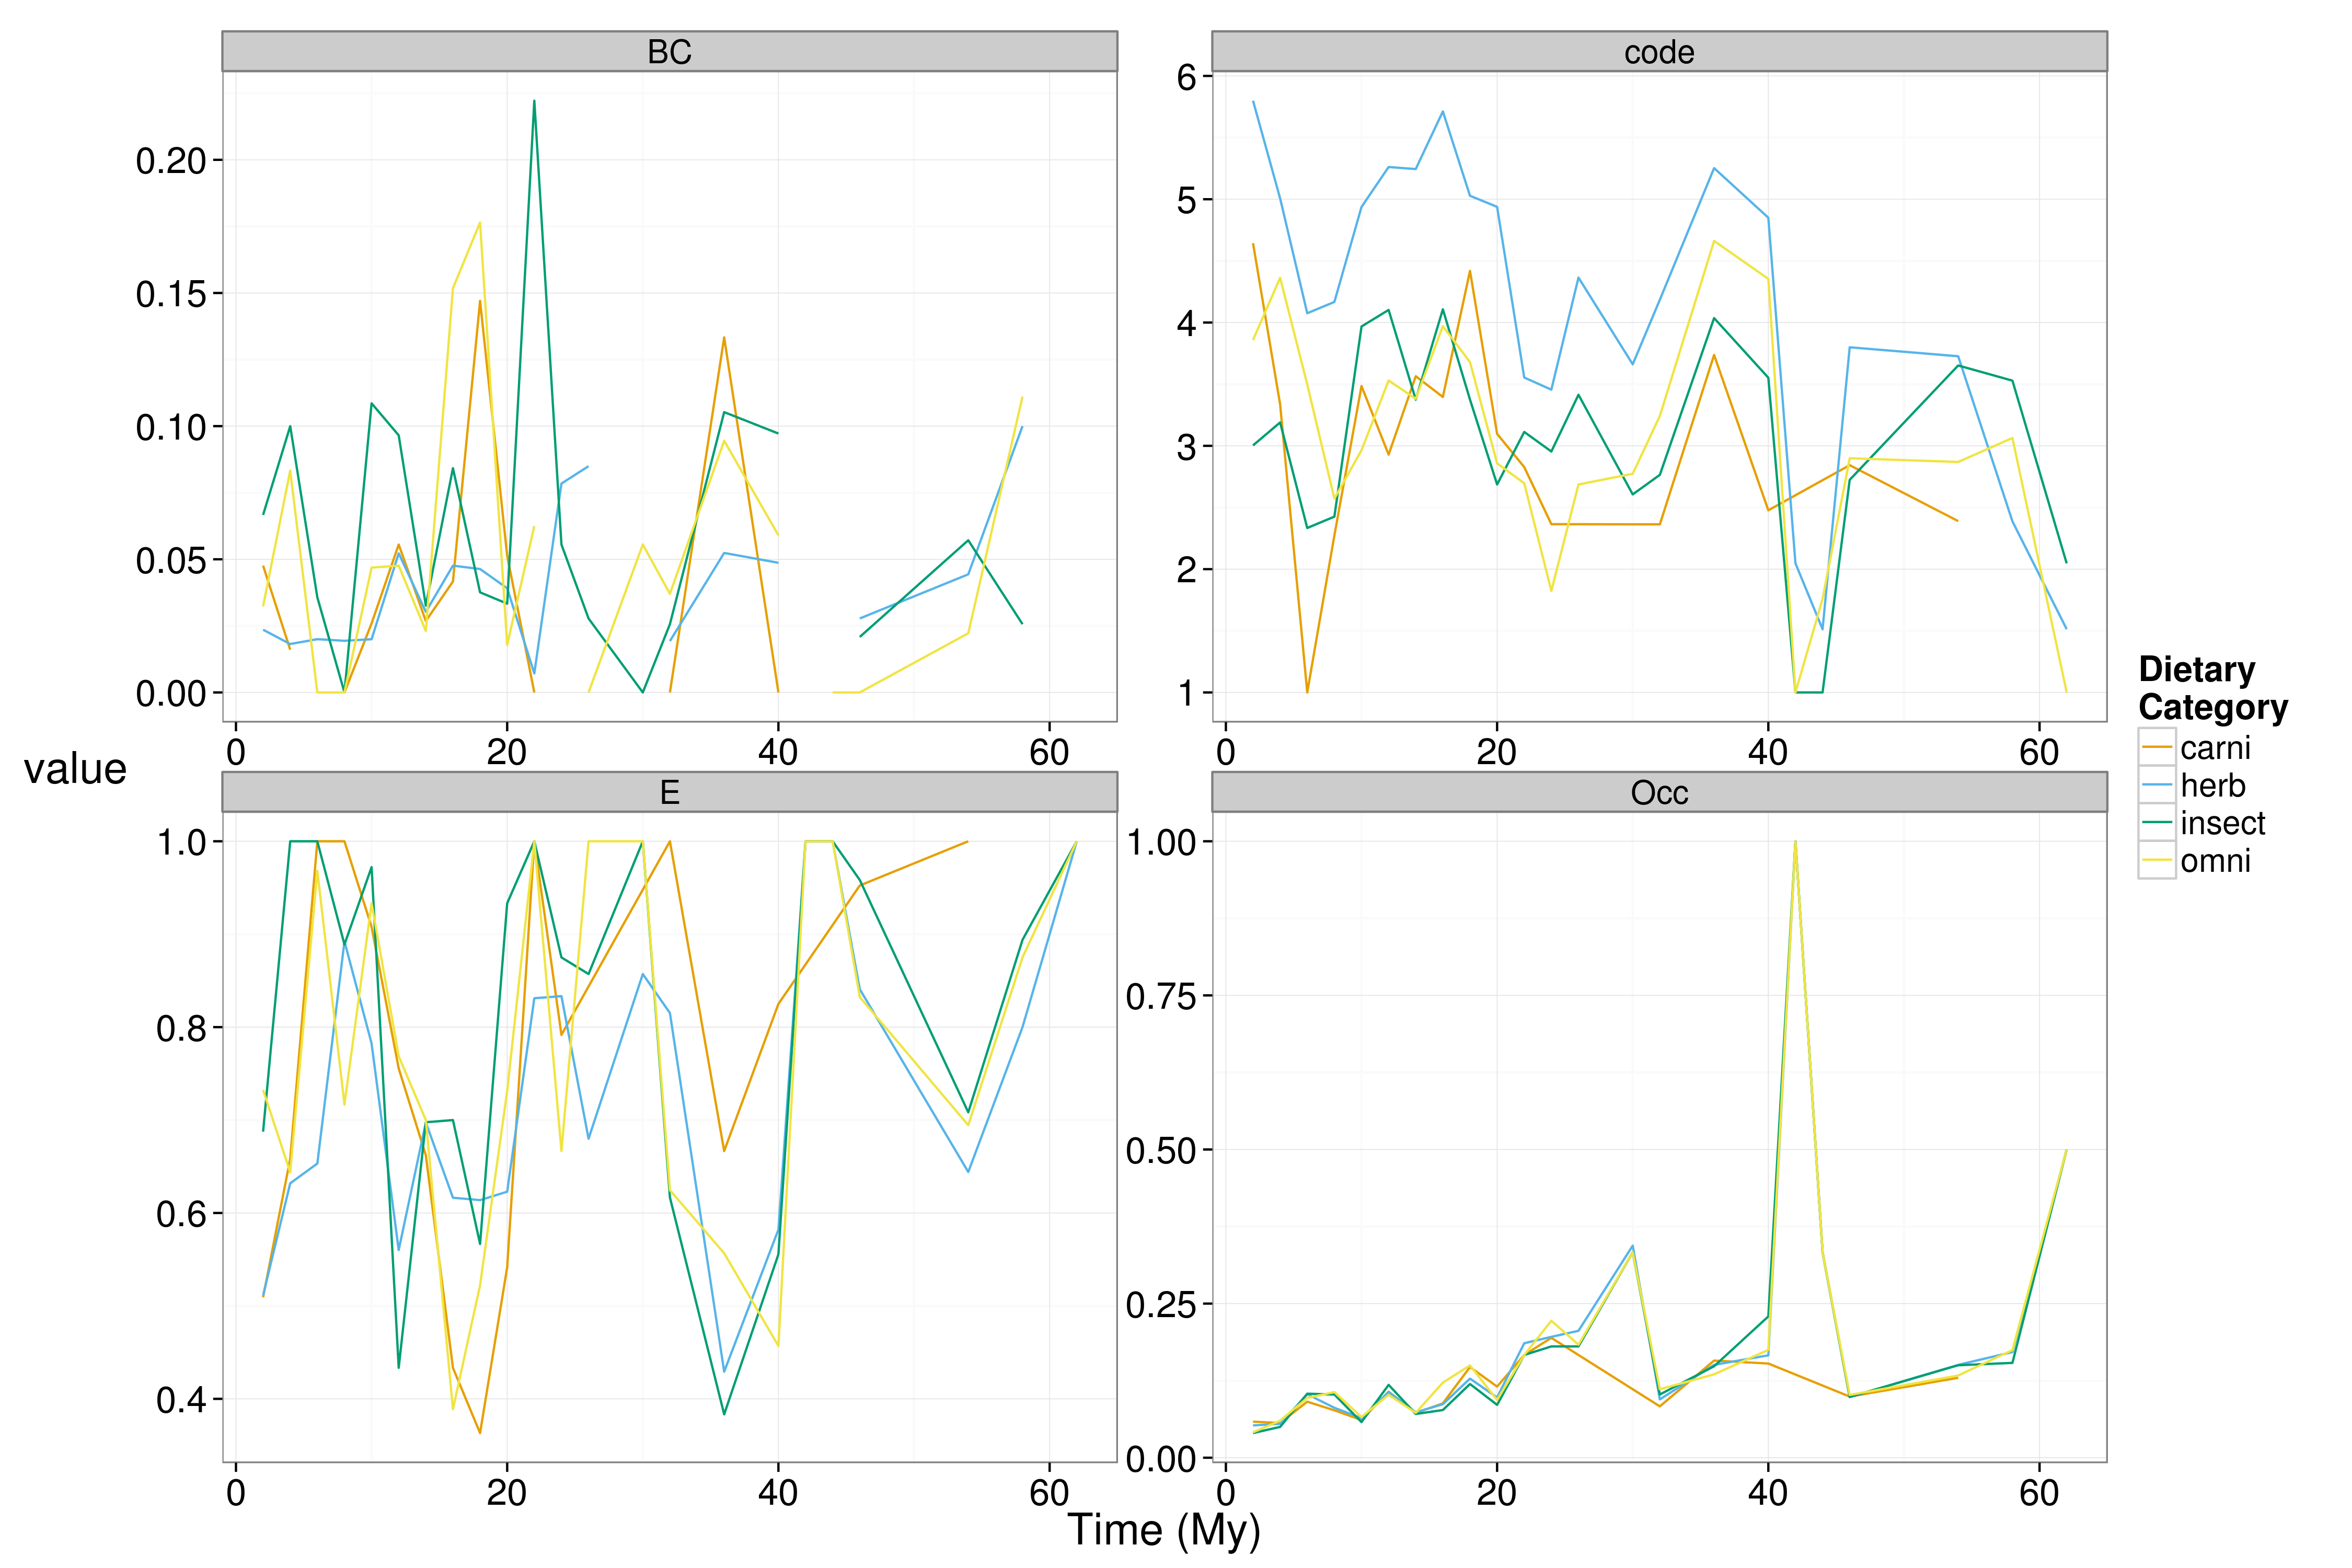
\includegraphics[height = 0.35\textheight, width = \textwidth, keepaspectratio = true]{figure/er_dt}
  \end{center}
\end{frame}


% summary
\begin{frame}
  \frametitle{Questions}

  \begin{alertblock}{Questions}
    \begin{itemize}
      \item Why do certain taxa go extinct while others do not?
      \item How is emergence ``formed?'' When should it be invoked?
      \item Is extinction risk taxon--age independent?
      \item When should we expect global, regional, or local processes to dominate?
    \end{itemize}
  \end{alertblock}
\end{frame}

\begin{frame}
  \frametitle{Summary of proposed research}

  \begin{alertblock}{Studies}
    \begin{itemize}
      \item Permian brachiopod trait based survival %\\(environmental preference)
      \item Cenozoic mammal trait based survival %\\(range size)
      \item Cenozoic mammal community connectedness %\\(global versus regional versus local)
    \end{itemize}
  \end{alertblock}

\end{frame}


% end
\begin{frame}
  \frametitle{Acknowledgements}
  \begin{columns}
    \begin{column}{0.5\textwidth}
      \begin{itemize}
        \item \textbf{Committee}
          \begin{itemize}
            \item Kenneth D. Angielczyk (co-advisor)
            \item Michael J. Foote (co-advisor)
            \item P. David Polly
            \item Richard H. Ree
          \end{itemize}
        \item Discussion
          \begin{itemize}
            \item David Bapst, Megan Boatright, Ben Frable, Colin Kyle, Darcy Ross, Liz Sander
            \item John Alroy, Graeme Lloyd, Carl Simpson, Graham Slater
          \end{itemize}
      \end{itemize}
    \end{column}
    \begin{column}{0.5\textwidth}
      
\includegraphics[height = 0.25\textheight, keepaspectratio = true]{figure/chicago} \\
      
\includegraphics[height = 0.25\textheight, width = 0.5\textwidth, keepaspectratio = true]{figure/field} \\
    \end{column}
  \end{columns}
\end{frame}


%\begin{frame}
%  \frametitle{Theseus' ship}
%  \begin{quotation}
%    The ship wherein Theseus and the youth of Athens returned from Crete had thirty oars, and was preserved by the Athenians down even to the time of Demetrius Phalereus, for they took away the old planks as they decayed, putting in new and stronger timber in their place, in so much that this ship became a standing example among the philosophers, for the logical question of things that grow; one side holding that the ship remained the same, and the other contending that it was not the same.

%    \attrib{Plutarch, \textbf{Theseus}}
%  \end{quotation}
%\end{frame}

\end{document}
